%% Please fill in your name and collaboration statement here.
\newcommand{\studentName}{**FILL IN YOUR NAME HERE**}
\newcommand{\collaborationStatement}{**FILL IN YOUR COLLABORATION STATEMENT HERE \\ (See the syllabus for information)**}


%%%%%%%%%%%%%%%%%%%%%%%%%%%%%%%%%%%%%%%%%%%%%%%
\documentclass[solution, letterpaper]{cscie121}
\usepackage{enumerate}
\usepackage{enumerate}
\usepackage{tikz}
\usepackage{pgf}
\usepackage{tikz}
\usetikzlibrary{arrows,automata}
\usepackage{hyperref}
\usetikzlibrary{automata,positioning}

\begin{document}
\header{3}{Friday, October 9, 2015}

\textbf{Important Note: You must redownload cscie121.cls from Canvas for this problem set, or your .tex will not compile. }


\problem{3+3+3+3+3+3} {3/4 page}
For each of the following languages, state whether the language is regular or non-regular. If regular, state a regular expression that denotes the language. If non-regular, write a short proof to justify.

\subproblem \{$xyx^R : x, y \in \Sigma^*$ \}
\subproblem \{$a^ib^ja^jb^i$: $i$, $j\geq0$\}.
\subproblem
$\{w\;:\;\textrm{$w$ is, for some $n\geq 1$, the decimal notation
for $10^n$}\}$. 
\subproblem $\{a^{2n}b^{n}: n\geq 0\}$
\subproblem $\{a^nb^n : n \geq 0$ and $n \neq 3i+5j$ for any $i \in \mathbb{N}, j \in \mathbb{N} \}$ Hint: Try explicitly working out all the strings in the language.
\subproblem $\{R\;:\;\textrm{$R$ is a regular expression for a
language over $\Sigma$}\}$ for some alphabet $\Sigma$.

\begin{solution}
  % Write your answer here.
\end{solution}

\problem{2+4} {1/2 page}

\subproblem
A context-free grammar $G$ is ambiguous if there exists a
string $w \in L(G)$ with two distinct leftmost derivations in $G$. Show that the context-free grammar $G = (V, \Sigma, R, S)$, where
$V=\{S,A,a,b\}$, $\Sigma = \{a,b\}$, and $R = \{S \rightarrow AA, A
\rightarrow AAA, A \rightarrow bA, A \rightarrow Ab, A \rightarrow a\}$
is ambiguous, because $aba$ has two different leftmost derivations in 
$G$.

\subproblem
Prove that $L(G)$,
where $G$ is the context-free grammar in Part (A), is regular.


\begin{solution}
  % Write your answer here.
\end{solution}


\problem{3+3+2}{3/4 page}
$$ L_1 = \{a^nb^m : m,n \geq 0 , m \neq n\} $$
$$ L_2 =  \{a^nb^ma^mb^n : m,n \geq 0\} $$


\subproblem Construct a context-free grammar $G_1$ for $L_1$
\subproblem Construct a context-free grammar $G_2$ for $L_2$.
\subproblem Construct a context-free grammar for $L_1L_2$.

\begin{solution}
  % Write your answer here.
\end{solution}


\problem{$3+3+(2)$}{$\frac12$ page}
An \emph{arithmetic progression} is a set of the form $\{p+qn \,:\, n \in \Nat\}$ for some $p,q \in \Nat$. For example, the set $\{10,13,16,19,\ldots\} = \{10+3n \,:\, n \in \Nat\}$ is an arithmetic progression.

\subproblem  Show that if $L \subseteq a^*$ and $\{|w| \,:\, w \in L\}$ is an arithmetic progression, then $L$ is regular. (An example of such a language $L$ is the language $\left\{a^{10+3n} \,:\, n \in \Nat\right\}$.)

\subproblem Use a counterexample to show that if $L \subseteq \{a,b\}^*$ and $\{|w| : w \in L\}$ is an arithmetic progression, then $L$ need not be regular.

\subproblem (Challenge!! Not required; worth up to 2 extra credit points.) Let $S \subseteq \Nat$ be an infinite set that does not contain any arithmetic progression as a subset. Let $L$ be an infinite language and $L \subseteq \{w \in \Sigma^* \,:\, |w| \in S\}$. (In other words. $\forall w \in L$, $|w| \in S$.) Prove that $L$ is not regular.\\\\
\textit{Note: On every problem set we will provide a challenge problem, generally significantly more difficult than the other problems in the set, but worth only a few points. It is recommended that you attempt these problems, but only after completing the rest of the assignment.}

\begin{solution}
  % Write your answer here.
\end{solution}





\problem{4}{$\frac14$ page}
Define an \emph{arithmetic function} as any function $\Nat \to \Nat$. Use a diagonalization argument to prove that the set of arithmetic functions is uncountably infinite.

\begin{solution}
  % Write your answer here.
\end{solution}


\problem{4+2}{1/2 page}

Let $\Sigma$ be some alphabet. Consider $L = \{ R : R \text{ is a regular expression for a language over} \Sigma \}$. 

\subproblem Prove that L is not a regular language. 
\subproblem Give a context-free grammar which generates L. 
 
\begin{solution}
  % Write your answer here.
\end{solution}

\problem{6}{1/2 page}
An {\em All-Paths-NFA} is exactly the same as an NFA except 
that it is defined to accept a string $x$ only if {\em all} computation 
paths on $x$ end in an accept state and rejects $x$ otherwise. 
(In contrast, a standard NFA accepted a string if {\em any} 
computation path leads to an accepting state). Show that a language 
$L$ 
is regular if and only if it is recognized by some All-Paths-NFA. 

For example, given the NFA:
\begin{center}
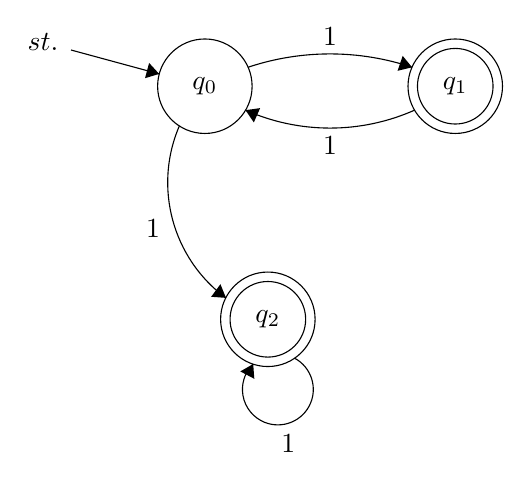
\begin{tikzpicture}[scale=0.2]
\tikzstyle{every node}+=[inner sep=0pt]
\draw [black] (12.6,-28.5) circle (3);
\draw (12.6,-28.5) node {$q_0$};
\draw [black] (28.5,-28.5) circle (3);
\draw (28.5,-28.5) node {$q_1$};
\draw [black] (28.5,-28.5) circle (2.4);
\draw [black] (16.6,-43.3) circle (3);
\draw (16.6,-43.3) node {$q_2$};
\draw [black] (16.6,-43.3) circle (2.4);
\draw [black] (4.1,-26.2) -- (9.7,-27.72);
\draw (3.33,-25.68) node [left] {$st.$};
\fill [black] (9.7,-27.72) -- (9.06,-27.02) -- (8.8,-27.99);
\draw [black] (15.343,-27.295) arc (108.4786:71.5214:16.429);
\fill [black] (25.76,-27.3) -- (25.16,-26.57) -- (24.84,-27.52);
\draw (20.55,-25.95) node [above] {$1$};
\draw [black] (25.92,-30.018) arc (-66.02452:-113.97548:13.216);
\fill [black] (15.18,-30.02) -- (15.71,-30.8) -- (16.11,-29.89);
\draw (20.55,-31.66) node [below] {$1$};
\draw [black] (13.939,-41.945) arc (-126.42784:-203.32414:9.107);
\fill [black] (13.94,-41.94) -- (13.59,-41.07) -- (13,-41.87);
\draw (9.79,-37.51) node [left] {$1$};
\draw [black] (18.288,-45.766) arc (62.1301:-225.8699:2.25);
\draw (17.9,-50.58) node [below] {$1$};
\fill [black] (15.67,-46.14) -- (14.85,-46.61) -- (15.74,-47.08);
\end{tikzpicture}
\end{center}

The string ``11111'' would be accepted, while ``1111'' would be rejected. 
\\\\
\begin{solution}
  % Write your answer here.
\end{solution}




\end{document}
